\section{Integralregning} \label{mat:sec:intergral}
Nu ved vi, hvordan man finder hastighed og acceleration ud fra positionen, men hvis man nu kender hastigheden eller accelerationen, og man gerne vil finde positionen, hvad gør man så?
Vi har brug for det omvendte af differentialregning, hvilket hedder integralregning. Det er dog lidt sværere, end differentialregning. Det skyldes, at flere \emph{forskellige} funktioner, kan have den \emph{samme} afledte. Et eksempel på dette er
%
\begin{align} \label{mat:eq:sum_func_const_deriv}
    \dv{f}{t}= \dv{}{t} \Big( f(t)+k \Big),
\end{align}
%
hvor $k$ er en konstant. At \cref{mat:eq:sum_func_const_deriv} kan ses ved at bruge sumreglen og \cref{mat:tab:diff}. Har vi en funktion med en bestemt afledt, kan vi altid finde en ny funktion med den samme afledte ved at lægge en konstant til funktionen.

Hvis vi har en funktion, $f(t)$, er den afledte funktion af $f(t)$, den funktion man får, når man differentierer $f(t)$. Tilsvarende er en \emph{stamfunktion}, $F(t)$, for funktionen $f(t)$, en funktion, der har den egenskab, at dens afledte er lig med den oprindelige funktion $f(t)$. En stamfunktion $F(t)$ er altså defineret til at opfylde
%
\begin{align}
    \dv{F}{t} &= f(t).
    %
    \intertext{Man finder stamfunktioner med det \emph{ubestemte integral}, som skrives}
    %
    \int f(t) \dd{t} &= F(t)+k.
\end{align}
%
Stamfunktionerne for de fleste simple funktioner kan med lidt snilde lures fra \cref{mat:tab:diff}, eller de kan ses i \cref{mat:tab:integral}.
%
\setlength{\tabcolsep}{1.2 em}
\def\arraystretch{1.5}
\begin{table}[]
    \centering
    \begin{tabular}{ccc}
    \toprule
    Funktionsnavn & $f(t)$ & $\displaystyle\int f(t)\dd{t}$ \\%\specialrule{.125em}{.1em}{.1em}
    \midrule
    Konstant & $k$ & $kt$ \\%\hline
    Potensfunktion & $t^n$ & $t^{n+1}/(n+1)$ \\%\hline
    Reciprokfunktion & $1/t$ & $\ln|t|$ \\%\hline
    Sinus & $\sin(t)$ & $-\cos(t)$ \\%\hline
    Cosinus & $\cos(t)$ & $\sin(t)$ \\%\hline
    Eksponentialfunktionen & $e^{kt}$ & $e^{kt}/k$ \\%\hline
    Den naturlige logaritme & $\ln(t)$ & $t\ln(t)-t$ \\
    % \specialrule{.125em}{.1em}{.1em}
    \bottomrule
    \end{tabular}
    \caption{Stamfunktioner for nogle af de mest almindelige funktioner, hvor det er undladt at lægge en tilfældig konstant til stamfunktionen. Bemærk at reglen for potensfunktioner ikke gælder, når $n=-1$.}
    \label{mat:tab:integral}
\end{table}

\begin{example}[Frit fald] \label{mat:ex:frit_fald}%
En af de simpleste fysiske situationer vi kan se på, er det frie fald.
Her er accelerationen konstant og lig med gravitationskonstanten
%
\begin{align*}
    a=g.
\end{align*}
%
Da man som tidligere nævnt finder accelerationen ved at differentiere hastigheden, \cref{mat:eq:acceleration}, må det også gælde, at hastigheden er en stamfunktion for accelerationen. Vi finder da hastigheden ud fra \cref{mat:tab:integral} til at være
%
\begin{align*}
    v = \int a \dd{t} = \int g \dd{t} = gt + v_0,
\end{align*}
%
hvor $v_0$ er konstanten for det ubestemt integral, der her angiver starthastigheden i det frie fald, altså hastigheden til tiden $t=0$. Vi finder da, at hastigheden vokser lineært med tiden.

Ligesom da vi differentierede, kan vi integrere mere komplicerede funktioner ved at tænke på dem som sammensætningere af simplere funktioner og benytte nogle regneregler for integralregning.
Integralet af en sum af funktioner er summen af deres integraler:
%
\begin{align}
    \int f(t)+g(t)\dd{t} &= \int f(t)\dd{t} + \int g(t)\dd{t}. \label{mat:eq:integral_sumregel}
    %
    \intertext{Tilsvarende kan vi sætte konstanter udenfor integraler:}
    %
    \int kf(t)\dd{t} &= k\int f(t)\dd{t}. \label{mat:eq:konstant}
\end{align}
%
Med disse basale integrationsregler\footnote{Det er også muligt at håndtere produktet af funktioner (delvis integration) og funktioner af funktioner (integration ved substitution), men det er mere kompliceret end de tilsvarende tekniker for differentialregning.} kan vi også finde positionen i vores eksempel
%
\begin{align} \label{mat:eq:position}
    x=\int v\dd{t}=\int gt+v_0\dd{t}=\frac{1}{2}gt^2+v_0t+x_0,
\end{align}
%
hvor $x_0$ her er positionen til tiden $t=0$.
\end{example}

\begin{figure}[]
    \centering
    \begin{tikzpicture}[line width=2pt]
        %
        \filldraw [draw=blue, fill=blue!25, line width=1.5pt]
            (2,0) rectangle (4,{4*(1/15 + 4/32) + 1});
        \filldraw [draw=red, fill=red!25, line width=1.5pt]
            (2,0) rectangle (4,{2*(1/15 + 2/32) + 1});
        \fill [gray!20, domain=2:4, pattern = north east lines, variable=\x]
            (2, 0) -- plot ({\x}, {\x*(1/15 + \x/32) + 1}) -- (4, 0) -- cycle;
        %
        \draw [domain=0:6.1] plot ({\x}, {\x*(1/15 + \x/32) + 1});
        \draw [-{Stealth[length=4mm, width=2.5mm]}] (0,0) to (6.5,0);
        \draw [-{Stealth[length=4mm, width=2.5mm]}] (0,0) to (0,3.5);
        %
        \draw (6.3,-0.1) node[anchor=north]{\huge $x$};
        \draw (-0.1,3.2) node[anchor=east]{\huge $y$};
        \draw (5.9,2.4) node[anchor=south east]{\huge $f(x)$};
        %
        \draw [{Stealth[length=2mm, width=2mm]}-{Stealth[length=2mm, width=2mm]}]
            (2,2) to (4,2);
        \draw (3,2.05) node[anchor=south]{\huge $\Delta x$};
        %
        \draw (2,-0.15) node[anchor=north]{\LARGE $x$};
        \draw (4,-0.025) node[anchor=north]{\LARGE $x + \Delta x$};
    \end{tikzpicture}
    %
    % 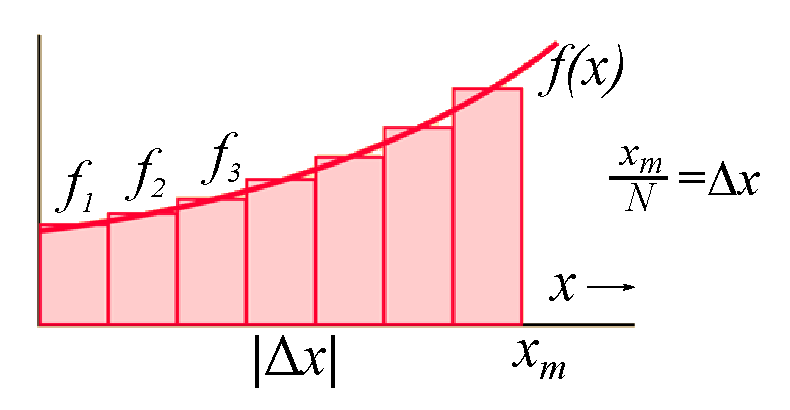
\includegraphics[width = 0.7\textwidth]{matfig/integral.eps}
    \caption{Arealet under grafen $f(x)$ i intervallet $[x,x+\Delta x]$ er skraveret, mens en rød og en blå rektangel viser en tilnærmelse af det skraverede areal. Man skal forestille sig, at det blå rektangel går helt ned til $x$-aksen ligesom den røde. I dette tilfælde er arealet af det røde rektangel mindre end arealet af det blå.}
    \label{mat:fig:areal_under_graf}
\end{figure}
%
\subsection{Integraler og arealet under en graf} \label{mat:subsec:int}
Ligesom differentialkvotienter (afledte funktioner) giver hældningen af grafen for en funktion, er der også en grafisk fortolkning af integraler.
Lad os sige, at vi har en funktion $A(x)$, der giver os arealet under en graf $f(x)$ målt fra $x=0$. Kigger man på arealet under grafen for $f(x)$ i et interval $[x,x+\Delta x]$ på $x$-aksen, vil arealet være givet ved $A(x+\Delta x) - A(x)$. Dette areal må være næsten det samme som arealet af en firkant med højden $f(x)$ og bredten $\Delta x$, men også firkanten med højden $f(x+\Delta x)$ og bredten $\Delta x$. Dette er illustreret i \cref{mat:fig:integralapprox}, hvor firkanten med højden $f(x)$ er tegnet med rød, og den med højden $f(x+\Delta x)$ i blå. Det præcise areal er skraveret. Fra figuren ses det at\footnote{Den aktive læser kan overveje, hvad man skal gøre, for at få udregningerne til at passe, hvis $f(x + \Delta x) \geq f(x)$ eller begge farvede arealer er enten større eller mindre end det skraverede.}
%
\begin{align} \label{mat:eq:int_ulighed}
    f(x)\Delta x \leq A(x+\Delta x) - A(x) \leq f(x+\Delta x) \Delta x.
\end{align}
%
\Cref{mat:eq:int_ulighed} fortæller med symboler, at det røde areal er mindre end det skraverede, som så er mindre end det blå. Divideres med $\Delta x$ i \cref{mat:eq:int_ulighed} fås
%
\begin{align} \label{mat:eq:int_ulighed2}
    f(x) \leq \frac{A(x+\Delta x) - A(x)}{\Delta x} \leq f(x+\Delta x).
\end{align}
%
Kigger man på \cref{mat:eq:diffkvotient} ses det, at der blot mangler en grænseværdi i \cref{mat:eq:int_ulighed2}, for at få den afledte af arealfunktionen imellem de to ulighedstegn. Tages grænseværdien for $\Delta x \rightarrow 0$ i \cref{mat:eq:int_ulighed2} fås\footnote{Skal man være helt stringent, så må man antage, at $f(x)$ er en kontinuert funktion, for at grænseværdien $\lim_{\Delta x\rightarrow 0} f(x+\Delta x)$ eksisterer. Det er sådan noget, der er meget vigtigt i universitetsmatematik.}
%
\begin{align} \label{mat:eq:int_ulighed3}
    \lim_{\Delta x\rightarrow 0} f(x) \leq \lim_{\Delta x\rightarrow 0} \frac{A(x+\Delta x) - A(x)}{\Delta x} \leq \lim_{\Delta x\rightarrow 0} f(x+\Delta x) \implies f(x) \leq \dv{A}{x} \leq f(x)
\end{align}
%
Da $\dv*{A}{x}$ ikke både kan være større end og mindre end $f(x)$ på samme tid, må der gælde lighedstegn begge steder. Det vil sige at
%
\begin{align}
    \dv{A}{x} = f(x).
\end{align}
%
Derfor må arealfunktionen, $A(x)$, være en stamfunktion til $f(x)$: $A(x) = F(x)$. Man kan derfor bruge stamfunktioner til at bestemme arealet under en graf. Siden den eneste forskel imellem forskellige stamfunktioner er en konstant, og da arealet under grafen i et bestemt interval på $x$-aksen udregnes som en forskel, vil konstanten forsvinde\footnote{Hvis det ikke er klart, hvorfor dette er sandt, så kan man se \cref{mat:ex:best_int}.}, og det er ligegyldigt, hvilken stamfunktion vi bruger.
Notationsmæssigt skrives arealet imellem $x_1$ og $x_2$ under grafen for $f(x)$ som
%
\begin{align} \label{mat:eq:best_int}
    A(x_1,x_2) = \int_{x_1}^{x_2}f(x)\dd{x} = F(x_2)-F(x_1),
\end{align}
%
hvor
%
\begin{align}
    \dv{F}{x} = f(x).
\end{align}
%
Her skriver man ofte forskellen mellem stamfunktionen i grænserne som
%
\begin{align} \label{mat:eq:klammestamfunktion}
    F(x_2)-F(x_1) = \Big[F(x)\Big]_{x_1}^{x_2},
\end{align}
%
hvilket er smart i praksis, da man så kan håndtere det ubestemte integral først, og herefter indsætte grænserne.

\begin{figure}[]
    \centering
    \begin{tikzpicture}[line width=2pt]
        %
        \foreach \i in {0,...,7}
        {
        % \filldraw[draw=blue, fill=blue!25, line width=1.5pt]
        %     (\i,0) rectangle (\i+1,{(\i+1)*(1/15 + (\i+1)/32) + 1});
        \filldraw[draw=red, fill=red!25, line width=1.5pt]
            (\i,0) rectangle (\i+1,{\i*(1/15 + \i/32) + 1});
        }
        %
        \draw [domain=0:8.6] plot ({\x}, {\x*(1/15 + \x/32) + 1});
        \draw [-{Stealth[length=4mm, width=2.5mm]}] (0,0) to (9,0);
        \draw [-{Stealth[length=4mm, width=2.5mm]}] (0,0) to (0,4.5);
        %
        \draw (8.8,-0.1) node[anchor=north]{\huge $x$};
        \draw (-0.1,4.3) node[anchor=east]{\huge $y$};
        \draw (8.3,3.85) node[anchor=north west]{\huge $f(x)$};
        %
        \draw[{Stealth[length=2mm, width=2mm]}-{Stealth[length=2mm, width=2mm]}]
            (3,-0.25) to (4,-0.25);
        \draw (3.5,-0.275) node[anchor=north]{\huge $\Delta x$};
    \end{tikzpicture}
    %
    % 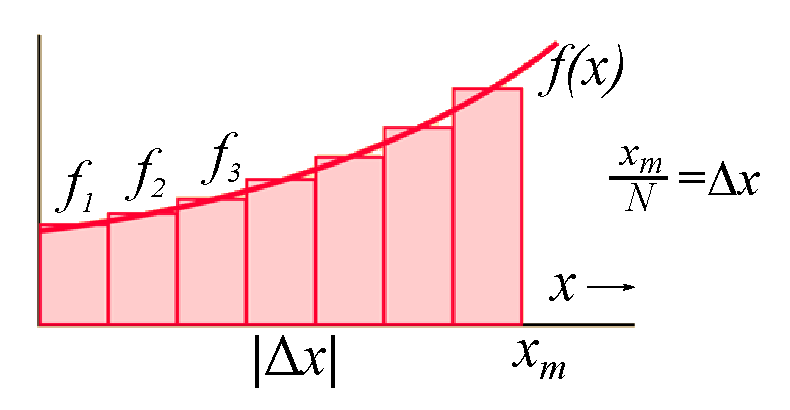
\includegraphics[width = 0.7\textwidth]{matfig/integral.eps}
    \caption{Arealet under grafen $f(x)$ tilnærmet ved at dele det op i rektangler. Det præcise integral fås så i grænsen hvor $\Delta x$ går mod $0$. Figuren er inspireret af \cite{Integral}.}
    \label{mat:fig:integralapprox}
\end{figure}
%
Notationen til integraler kommer netop fra idéen om at beskrive arealet under en graf.
Siden vi ved, hvordan man udregner arealet på et rektangel, kan arealet under funktionen estimeres ved at dele det op i rektangler, som er illustreret i \cref{mat:fig:integralapprox}.
Gør man det, og lægger alle arealerne sammen, får man at arealet
%
\begin{align} \label{mat:eq:finitesum}
    A \approx \sum_{i=1}^m f(x_i)\Delta x,
\end{align}
%
hvor $\sum$ er et sumtegn. Her er $i$ et indeks, der bliver fastsat i bunden, og som så går op i skridt af 1 indtil $i$ bliver lig $m$, der står over sumtegnet. Altså har man f.eks. at
%
\begin{align}
    \sum_{i=1}^m i &= 1 + 2 + 3 + \dots{} + m,
    %
    \intertext{og}
    %
    \sum_{i=1}^m f(x_i) &= f(x_1) + f(x_2) + \dots{} + f(x_m).
\end{align}
%
Gøres $\Delta x$ nu mindre og mindre i \cref{mat:eq:finitesum}, bliver tilnærmelsen bedre og bedre, så som i differentialregning lader vi $\Delta x$ gå imod nul og får at
%
\begin{align}
    A = \lim_{\Delta x\rightarrow 0} \sum_{i=1}^m f(x_i)\Delta x
    = \int_{x_1}^{x_m} f(x) \dd{x}.
\end{align}
%
Dette er den typiske måde at definere et integral\footnote{Dette kaldes for et Riemannintegral efter den tyske matematiker Bernhard Riemann. Der eksisterer også andre måder at definere integralet, men det er ikke vigtigt til vores formål.}. Integraltegnet $\int$ er derfor et kunstfærdigt S, som kommer af, at der er tale om en ``sum''.

% \subsubsection{Eksempel}
\begin{example} \label{mat:ex:best_int}%
For at illustrere hvordan man løser et bestemt integral, vil vi nu finde det bestemte og ubestemte integral af funktionen $f(x) = 15x^2 + e^x$. For det ubestemte integral finder man at
%
\begin{align*}
    \int f(x) \dd{x} = \int 15x^2 + e^x \dd{x} = \int 15x^2 \dd{x} + \int e^x \dd{x} = 15 \int x^2 \dd{x} + \int e^x \dd{x},
\end{align*}
%
hvor vi har benyttet, at vi må dele integralet op i to integraler og flytte en konstant udenfor. Vi mangler dog stadig en konstant, men vi får en konstant fra hver af de to integraler:
%
\begin{align*}
    \int x^2 \dd{x} &= \frac{1}{3} x^3 + C_1,
    %
    \intertext{og}
    %
    \int e^x \dd{x} &= e^x + C_2,
\end{align*}
%
Her er det antaget, at de to integrationskonstanter kan være forskellige. Samles det hele nu finder man resultatet:
%
\begin{align*}
    \int f(x) \dd{x} = 15\left( \frac{1}{3} x^3 + C_1 \right) + \left( e^x + C_2 \right) = 5x^3 + 15C_1 + e^x + C_2 = 5x^3 + e^x + C,
\end{align*}
%
hvor konstanterne i det sidste trin er samlet i den ene konstant $C=15C_1+C_2$, da både $C_1$ og $C_2$ bare er tilfældige konstanter. Nu ved vi, at enhver stamfunktion, $F(x)$, for $f(x)$ har formen $F(x) = 5x^3 + e^x + C$, og vi kan derfor beregne det bestemte integral fra $x=a$ til $x=b$ som følger
%
\begin{align*}
\int_a^b f(x) \dd{x} = \Big[F(x)\Big]_ a^b = \left[ 5x^3 + e^x + C \right]_a^b.
\end{align*}
%
Her ses det smarte ved notationen i \cref{mat:eq:klammestamfunktion}, idet det viser, at vi kan dele et bestemt integral op: først løses et ubestemt integral vha. \cref{mat:tab:integral} og regnereglerne i \cref{mat:eq:integral_sumregel,mat:eq:konstant}, for derefter at indsætte grænserne. Vi kan altså gøre en ting ad gangen. Nu kan vi så indsætte grænserne og få at
%
\begin{align*}
    \int_a^b f(x) \dd{x} = \left( 5b^3 + e^b + C \right) - \left( 5a^3 + e^a + C \right) = 5 \left( b^3 - a^3 \right) + \left( e^b - e^a \right).
\end{align*}
%
Som det ses her, har værdien af konstanten $C$ ikke nogen betydning for det bestemte integral og undlades derfor ofte ved beregninger. For god ordens skyld kan vi vælge nogle tal som vores grænser, for at se at et bestemt integral faktisk giver et tal og ikke en ny funktion, hvilket er nødvendigt for at det kan være et areal under kurven. For at gøre det let for os selv vælges grænserne $a=0$ og $b=1$, og vi får således at
%
\begin{align*}
    \int_0^1 f(x) \dd{x} = 5 \left( 1^3 - 0^3 \right) + \left( e^1 - e^0 \right) = 5 + e - 1 = 4 + e.
\end{align*}
%
Arealet under grafen for funktionen $f(x)$ i intervallet fra $0$ til $1$ er derfor $4+e$. Dette illustrerer også en vigtig forskel på det bestemte og det ubestemte integral -- det bestemte giver et tal, mens det ubestemte giver en funktion.
\end{example}